\section{Server Backend}
This chapter covers the core component of the iCare Server: The Server Backend. The following subchapters describe the architecture of the server with its individual components and the technologies used to implement communication between the subsystems.
\subsection{The Server architecture}
The following figure \ref{icare-serverarchitecure} shows the general architecture of the backend server and the external systems with which the server communicates at runtime. The focus here lies on the \textit{iCare Server} subsystem, while the other components of the system \textit{iCare Frontend}, \textit{iCare Room HUB}, \textit{iCare Backup System} and \textit{iCare Data} are treated as black boxes. 
\begin{figure}[H]
	\centering
	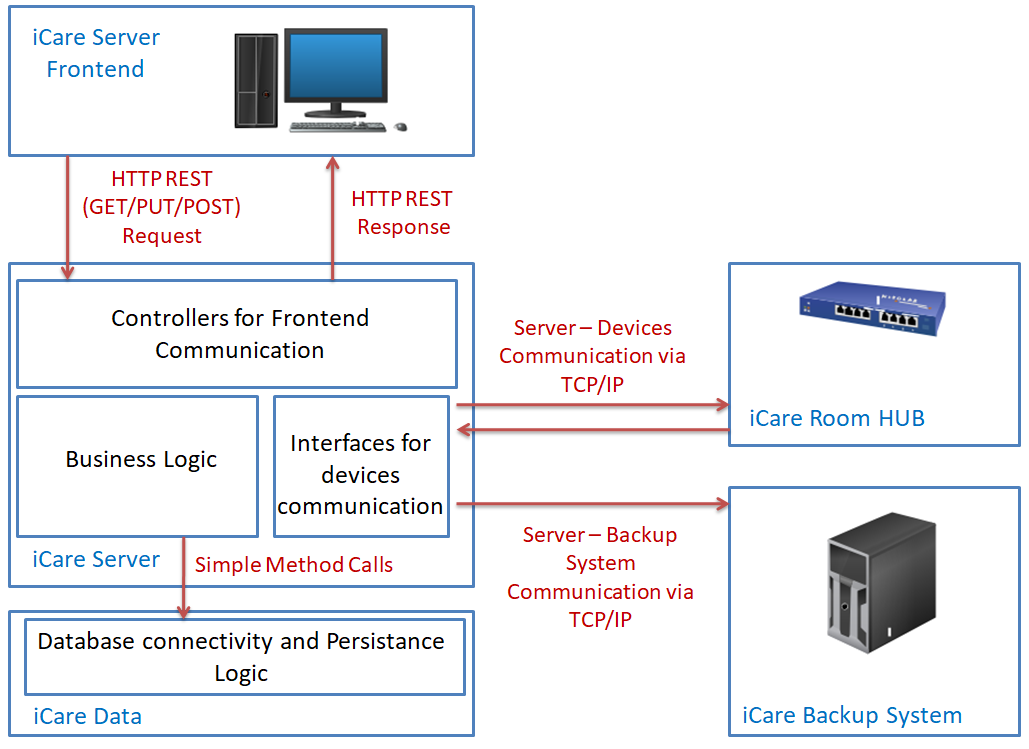
\includegraphics[width =1.0\textwidth]{images/server-architecture.PNG}
	\caption{iCare Server architecture}
	\label{icare-serverarchitecure}
\end{figure}
\subsection{Communication between frontend and backend via REST}
\subsection{Communication between Server and Devices/Backup system}
\subsection{Business Logic}
\subsection{Connection to ICare Data}